\documentclass[sigconf,nonacm]{acmart}

\setcopyright{none}
\settopmatter{printacmref=false}
\renewcommand\footnotetextcopyrightpermission[1]{}
\pagestyle{plain}

\usepackage{booktabs}
\usepackage{tabularx}
\usepackage{array}
\usepackage{graphicx}
\usepackage{amsmath}
\usepackage{tikz}
\usetikzlibrary{shapes.geometric,arrows.meta,positioning,fit,backgrounds,calc}
\usepackage{url}
\urlstyle{rm}

%% ── Colours ──────────────────────────────────────────────────────────────────
\definecolor{cblue}  {RGB}{ 70,120,200}
\definecolor{cgreen} {RGB}{ 60,160, 85}
\definecolor{corange}{RGB}{210,110, 30}
\definecolor{cpurple}{RGB}{130, 60,170}
\definecolor{cred}   {RGB}{200, 60, 50}
\definecolor{cgray}  {RGB}{100,100,100}
\definecolor{clb}    {RGB}{210,225,250}
\definecolor{clg}    {RGB}{205,240,210}
\definecolor{clo}    {RGB}{255,228,195}
\definecolor{clp}    {RGB}{235,210,250}
\definecolor{clr}    {RGB}{255,215,210}
\definecolor{clgy}   {RGB}{248,248,240}
\definecolor{cyellow}{RGB}{255,245,180}

\title{Threat Modeling Nation-State Attacks on Defense Contractors:
A DREAD-Based Risk Assessment Framework for Controlled Unclassified Information Protection}

\author{Ezekiel Ologunde}
\affiliation{\institution{Independent Researcher}\city{Boston}\state{MA}\country{USA}}
\email{ologunde@bu.edu}

\begin{abstract}
Small and medium defense contractors face asymmetric cybersecurity challenges: they
possess Controlled Unclassified Information (CUI) of strategic value to nation-state
adversaries while typically operating with resource constraints that limit defensive
capabilities. This paper presents a comprehensive threat modeling methodology employing
the DREAD (Damage, Reproducibility, Exploitability, Affected Users, Discoverability)
framework to assess nation-state threats targeting defense contractor email and
file-sharing infrastructure. Through analysis of two contemporary threat actor
profiles---Russian GRU-linked groups and the North Korean Lazarus Group---we
demonstrate how systematic risk assessment enables resource-constrained organizations
to prioritize security investments against advanced persistent threats. Applying DREAD
methodology to email and file server compromise scenarios, we quantify an aggregate risk
score of 8.0/10, driven by catastrophic damage potential (9/10), organization-wide user
impact (9/10), moderate-to-high exploitability (7--8/10), moderate-to-high
reproducibility (7/10), and moderate detection difficulty (5--6/10). The research
demonstrates that effective defense requires architectural approaches emphasizing
resilience over prevention, including identity governance, network segmentation,
comprehensive monitoring, rapid patch management, and multi-layered defense-in-depth
strategies. Our findings provide an actionable framework enabling defense contractors
to assess nation-state threats, justify security investments, prioritize architectural
improvements, and develop risk-informed strategies appropriate to their threat landscape
and resource constraints.
\end{abstract}

\begin{CCSXML}
<ccs2012>
  <concept>
    <concept_id>10002978.10003029</concept_id>
    <concept_desc>Security and privacy~Intrusion detection systems</concept_desc>
    <concept_significance>500</concept_significance>
  </concept>
  <concept>
    <concept_id>10002978.10003022</concept_id>
    <concept_desc>Security and privacy~Systems security</concept_desc>
    <concept_significance>500</concept_significance>
  </concept>
  <concept>
    <concept_id>10002978.10003006</concept_id>
    <concept_desc>Security and privacy~Threat modeling</concept_desc>
    <concept_significance>500</concept_significance>
  </concept>
</ccs2012>
\end{CCSXML}

\ccsdesc[500]{Security and privacy~Intrusion detection systems}
\ccsdesc[500]{Security and privacy~Systems security}
\ccsdesc[500]{Security and privacy~Threat modeling}

\keywords{Threat modeling; DREAD; nation-state threats; defense contractors; APT;
controlled unclassified information; GRU; Lazarus Group; risk assessment;
cybersecurity architecture}

\begin{document}
\maketitle

\subsection*{Methodological Disclosure.}
The DREAD scores reported here (Damage 9/10, aggregate risk 8.0/10, and the
component Reproducibility/Exploitability/Affected Users/Discoverability
ratings) are this author's own subjective qualitative judgment applied to
the DREAD rubric, not an empirically measured or independently validated
quantity; DREAD scoring is inherently a structured expert-opinion exercise,
and no statistical, measured, or third-party-validated data underlies these
numbers. Likewise, the cost-estimate table (Total Year~1: \$205K--\$600K;
Ongoing Year~2+: \$175K--\$450K) is a rough illustrative estimate assembled
from general market ranges for the listed security controls, not a vendor
quote, procurement analysis, or costed implementation plan for any real
organization. No real defense contractor engagement, incident data, or
threat-intelligence access informed these figures; the GRU- and
Lazarus-linked threat-actor profiles are drawn from public reporting, and
the risk scores and costs are this author's own estimation exercise,
presented for illustrative and pedagogical purposes.

%%──────────────────────────────────────────────────────────────────────────────
\section{Introduction}
%%──────────────────────────────────────────────────────────────────────────────

Small and medium defense contractors occupy a precarious position in the national
security ecosystem. While they possess CUI of strategic value to foreign
adversaries---including technical specifications, program plans, supply chain
relationships, and collaborative communications---they typically operate with resource
constraints that dramatically limit their defensive capabilities compared to major
defense primes or government agencies~\cite{gao2021defense}.

This asymmetry creates an attractive target profile for nation-state APT actors.
Rather than confronting the sophisticated defenses of Lockheed Martin, Raytheon, or DoD
networks directly, adversaries increasingly target smaller contractors as pathways to
valuable information or stepping stones enabling supply chain compromise of larger
entities~\cite{crowdstrike2024global}. The 2020 SolarWinds supply chain attack
demonstrated this strategy's effectiveness, enabling access to numerous high-value
government and private sector networks through compromise of a widely-used IT management
platform~\cite{smith2021solarwinds}.

The regulatory environment has intensified significantly. DoD's CMMC framework mandates
progressively rigorous cybersecurity practices for organizations handling CUI, with
contract eligibility dependent on certification~\cite{dod2024cmmc}. Simultaneously,
nation-state threat actors have accelerated targeting of the defense industrial base,
with documented campaigns by Chinese, Russian, North Korean, and Iranian APT
groups~\cite{cisa2024nationstate}.

\subsection{Research Questions and Contributions}

This paper addresses five critical questions: (RQ1)~What nation-state threat actors pose
the most significant risks to small defense contractors? (RQ2)~What TTPs do these
adversaries employ against defense contractor infrastructure? (RQ3)~How can DREAD be
applied to assess nation-state threats to email and file-sharing systems?
(RQ4)~What architectural controls are most effective for resource-constrained
organizations? (RQ5)~How can threat modeling justify security investments?

Our contributions include: (1)~analysis of two primary nation-state threat actors; (2)~
detailed examination of their TTPs; (3)~DREAD application yielding a quantitative risk
assessment; (4)~a proposed architectural framework for resource-constrained contractors;
and (5)~a methodology for translating threat intelligence into investment justification.

%%──────────────────────────────────────────────────────────────────────────────
\section{Background and Related Work}
%%──────────────────────────────────────────────────────────────────────────────

\subsection{Threat Modeling Methodologies}

\textbf{STRIDE}~\cite{shostack2014threat} categorizes threats into six types
(Spoofing, Tampering, Repudiation, Information Disclosure, Denial of Service, Elevation
of Privilege), excelling at threat identification during design but providing less
quantitative risk assessment.

\textbf{PASTA}~\cite{ucedavelez2015risk} provides a seven-stage methodology integrating
business objectives, technical requirements, and threat intelligence. Its
comprehensiveness makes it valuable for large organizations but potentially overwhelming
for small teams.

\textbf{DREAD}~\cite{meier2003dread} quantifies risk across five dimensions: Damage
potential, Reproducibility, Exploitability, Affected users, and Discoverability. Each
dimension receives a score (1--10), and aggregate scores enable prioritization. While
criticized for potential subjectivity, DREAD's quantitative approach facilitates risk
communication---critical for resource-constrained organizations.

\subsection{Controlled Unclassified Information}

NARA defines CUI as information requiring safeguarding pursuant to federal law or
regulation, but not classified under Executive Order~13526~\cite{nara2024cui}. Relevant
categories for defense contractors include technical data, contract information, export
controlled information (ITAR, EAR), and proprietary business information. NIST SP~800-171
establishes 110 security controls for protecting CUI in non-federal
systems~\cite{nist2024sp800171}; CMMC builds upon this through third-party assessment
and certification~\cite{dod2024cmmc}.

\subsection{Defense Industrial Base Threat Landscape}

Research documents sustained nation-state targeting of the defense industrial base.
Chinese APT groups (APT1, APT10, APT40, APT41) have conducted extensive intellectual
property theft~\cite{mandiant2023china}, with the 2023 Volt Typhoon campaign
demonstrating interest in pre-positioning within critical
infrastructure~\cite{cisa2024volt}. Russian GRU-linked groups have deployed destructive
malware including NotPetya and CaddyWiper~\cite{greenberg2021sandworm}. The Lazarus
Group conducts dual-purpose operations: defense espionage supporting weapons development
and financially-motivated crime~\cite{crowdstrike2024global}. Small business
cybersecurity research documents particular challenges of resource constraints, competing
priorities, skills gaps, and compliance burdens~\cite{chang2025mind}.

%%──────────────────────────────────────────────────────────────────────────────
\section{Threat Actor Analysis}
%%──────────────────────────────────────────────────────────────────────────────

\subsection{Russian GRU-Linked Groups}

Russia's GRU, specifically military intelligence unit 74455 (Sandworm), conducts
operations supporting Russian military and intelligence objectives~\cite{greenberg2021sandworm}.
Unlike SVR (foreign intelligence), GRU groups have demonstrated willingness to conduct
disruptive and destructive operations, including Ukraine power grid attacks (2015--2016),
NotPetya (\$10B+ global damages, 2017), and CaddyWiper deployment (2022--present) in the
Ukraine conflict context~\cite{cisa2024russia,crowdstrike2024global}. Key TTPs include
spear-phishing targeting administrators, credential theft via memory extraction and
password reuse exploitation, scanning for unpatched internet-facing systems, and
deployment of destructive wiper malware with anti-forensics
capabilities~\cite{greenberg2019notpetya}.

Strategic objectives against defense contractors encompass intelligence collection of
technical data, pre-positioning for potential future disruption, and using smaller
contractors as testing grounds for tactics before applying them to harder targets.

\subsection{North Korean Lazarus Group}

The Lazarus Group operates under North Korea's Reconnaissance General Bureau, conducting
operations that blend espionage with financially-motivated
cybercrime~\cite{crowdstrike2024global}. High-profile operations include the Sony
Pictures hack (2014), Bangladesh Bank heist (\$81M stolen, 2016), WannaCry ransomware
(200,000 systems in 150 countries, 2017), and sustained cryptocurrency exchange attacks.

\textbf{Operation Dream Job (2020--present)} is particularly relevant to defense
contractors~\cite{mascellino2025dreamjob}: engineers receive highly convincing fake job
offers from reputable aerospace companies; multi-week engagements build trust before
malware delivery through ostensible job description documents; compromise proceeds
undetected for weeks, enabling extensive CUI exfiltration. The March 2025 compromise of
a European aerospace contractor illustrates the campaign's continued
sophistication~\cite{mascellino2025dreamjob}.

Key TTPs include: elaborate social engineering via fabricated recruitment campaigns;
custom modular malware with anti-analysis capabilities; credential dumping and lateral
movement using valid credentials to blend with legitimate activity; staged data
exfiltration using legitimate cloud services and encrypted channels.

\subsection{Comparative Analysis}

Table~\ref{tab:comparison} summarizes TTP comparison. Despite different strategic
objectives---GRU primarily focused on disruption supporting Russian military goals,
Lazarus balancing espionage with revenue generation---both actors exploit unpatched
vulnerabilities and weak authentication, use spear-phishing and credential theft,
conduct lateral movement, and demonstrate high operational security and persistence.
The distinction is that GRU more frequently deploys destructive malware as a primary
objective, while Lazarus specializes in elaborate social engineering and data
exfiltration. For a small defense contractor, both represent sophisticated, persistent
adversaries capable of compromising email and file server infrastructure.

\begin{table}[h]
\caption{Comparison of GRU and Lazarus TTPs.}
\label{tab:comparison}
\small
\begin{tabularx}{\columnwidth}{@{}Xcc@{}}
\toprule
\textbf{TTP} & \textbf{GRU} & \textbf{Lazarus} \\
\midrule
Spear-Phishing       & High      & High      \\
Social Engineering   & Moderate  & Very High \\
Credential Theft     & High      & High      \\
Lateral Movement     & High      & High      \\
Destructive Malware  & Very High & Moderate  \\
Data Exfiltration    & High      & Very High \\
Persistence          & High      & Very High \\
Anti-Forensics       & High      & High      \\
\bottomrule
\end{tabularx}
\end{table}

%%
%% FIGURE 1 — Threat Actor Overview (two-column span)
%%
%% Two actor boxes side-by-side (each 6.0cm wide, gap 0.8cm) → 12.8cm total.
%% Target banner below spanning 13.0cm.  All within \textwidth ≈ 17.8cm  ✓
%%
\begin{figure*}[t]
\centering
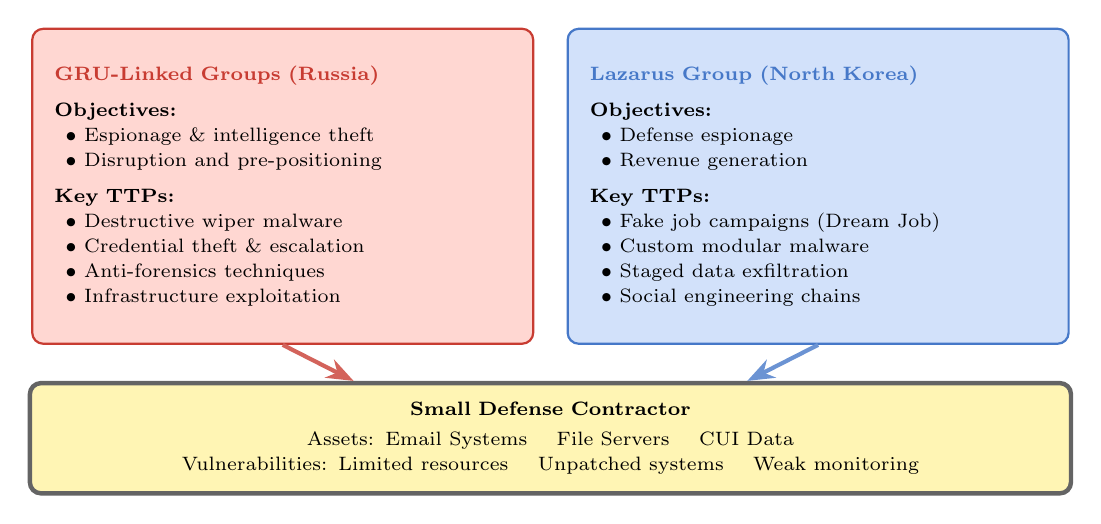
\begin{tikzpicture}[
  font=\fontsize{7pt}{9pt}\selectfont,
  >=Stealth,
  abox/.style={
    rectangle, rounded corners=4pt,
    minimum width=6.0cm, minimum height=4.0cm,
    text width=5.8cm, align=left,
    draw, thick, inner sep=8pt
  },
  tbox/.style={
    rectangle, rounded corners=4pt,
    minimum width=13.0cm, minimum height=1.4cm,
    text width=12.8cm, align=center,
    draw=cgray, ultra thick, fill=cyellow,
    font=\fontsize{7.5pt}{9pt}\selectfont,
    inner sep=6pt
  },
  arr/.style={-{Stealth}, line width=1.5pt}
]

  %% ── Left actor: GRU ───────────────────────────────────────────────────────
  \node[abox, fill=clr, draw=cred] (gru) at (-3.4, 0) {
    \textbf{\textcolor{cred}{GRU-Linked Groups (Russia)}}\\[4pt]
    \textbf{Objectives:}\\
    \hspace*{4pt}$\bullet$ Espionage \& intelligence theft\\
    \hspace*{4pt}$\bullet$ Disruption and pre-positioning\\[4pt]
    \textbf{Key TTPs:}\\
    \hspace*{4pt}$\bullet$ Destructive wiper malware\\
    \hspace*{4pt}$\bullet$ Credential theft \& escalation\\
    \hspace*{4pt}$\bullet$ Anti-forensics techniques\\
    \hspace*{4pt}$\bullet$ Infrastructure exploitation
  };

  %% ── Right actor: Lazarus ──────────────────────────────────────────────────
  \node[abox, fill=clb, draw=cblue] (laz) at (3.4, 0) {
    \textbf{\textcolor{cblue}{Lazarus Group (North Korea)}}\\[4pt]
    \textbf{Objectives:}\\
    \hspace*{4pt}$\bullet$ Defense espionage\\
    \hspace*{4pt}$\bullet$ Revenue generation\\[4pt]
    \textbf{Key TTPs:}\\
    \hspace*{4pt}$\bullet$ Fake job campaigns (Dream Job)\\
    \hspace*{4pt}$\bullet$ Custom modular malware\\
    \hspace*{4pt}$\bullet$ Staged data exfiltration\\
    \hspace*{4pt}$\bullet$ Social engineering chains
  };

  %% ── Target banner ─────────────────────────────────────────────────────────
  \node[tbox] (tgt) at (0, -3.2) {
    \textbf{Small Defense Contractor}\\[2pt]
    Assets: Email Systems \quad File Servers \quad CUI Data\\
    Vulnerabilities: Limited resources \quad Unpatched systems \quad Weak monitoring
  };

  %% ── Arrows ────────────────────────────────────────────────────────────────
  \draw[arr, color=cred!80]  (gru.south) -- ([xshift=-2.5cm]tgt.north);
  \draw[arr, color=cblue!80] (laz.south) -- ([xshift= 2.5cm]tgt.north);

\end{tikzpicture}
\caption{Two primary nation-state threat actors targeting small defense contractors.
  Both employ sophisticated TTPs against resource-constrained environments, though with
  different strategic objectives.}
\label{fig:actors}
\end{figure*}

%%──────────────────────────────────────────────────────────────────────────────
\section{DREAD Threat Model Analysis}
%%──────────────────────────────────────────────────────────────────────────────

We apply the DREAD framework to assess the threat of email and file server compromise
by nation-state actors. Figure~\ref{fig:dread} illustrates the five dimensions and
aggregate score.

%%
%% FIGURE 2 — DREAD Dimensions (single column)
%%
%% Five horizontal bars (6.0cm wide) + a score badge to the right.
%% Bar right edge: 3.0cm from centre. Badge centre at 4.7cm → right edge 5.6cm.
%% Total half-width ≈ 5.6cm  ✓  (column half ≈ 4.3cm … use figure* or tighter)
%% → Use single column, tighter bars: bar width=5.4cm, badge at 3.8cm right.
%%
\begin{figure}[h]
\centering
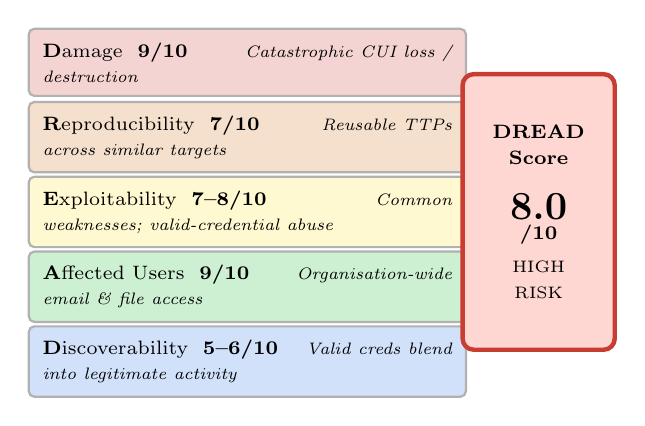
\begin{tikzpicture}[
  font=\fontsize{7pt}{9pt}\selectfont,
  >=Stealth,
  bar/.style={
    rectangle, rounded corners=2pt,
    minimum width=5.4cm, minimum height=0.78cm,
    text width=5.2cm, align=left,
    draw=cgray!50, thick,
    inner sep=5pt
  },
  badge/.style={
    rectangle, rounded corners=4pt,
    minimum width=1.8cm, minimum height=3.5cm,
    text width=1.65cm, align=center,
    draw=cred, ultra thick, fill=clr,
    font=\fontsize{7.5pt}{9.5pt}\selectfont\bfseries,
    inner sep=4pt
  }
]

  %% ── Five DREAD bars ──────────────────────────────────────────────────────
  \node[bar, fill=cred!22]    (d1) at (0, 0.00)
    {\textbf{D}amage\ \ \textbf{9/10} \hfill
     \fontsize{6.5pt}{8pt}\selectfont\itshape Catastrophic CUI loss / destruction};

  \node[bar, fill=corange!22] (d2) at (0,-0.95)
    {\textbf{R}eproducibility\ \ \textbf{7/10} \hfill
     \fontsize{6.5pt}{8pt}\selectfont\itshape Reusable TTPs across similar targets};

  \node[bar, fill=cyellow!60] (d3) at (0,-1.90)
    {\textbf{E}xploitability\ \ \textbf{7--8/10} \hfill
     \fontsize{6.5pt}{8pt}\selectfont\itshape Common weaknesses; valid-credential abuse};

  \node[bar, fill=clg]        (d4) at (0,-2.85)
    {\textbf{A}ffected Users\ \ \textbf{9/10} \hfill
     \fontsize{6.5pt}{8pt}\selectfont\itshape Organisation-wide email \& file access};

  \node[bar, fill=clb]        (d5) at (0,-3.80)
    {\textbf{D}iscoverability\ \ \textbf{5--6/10} \hfill
     \fontsize{6.5pt}{8pt}\selectfont\itshape Valid creds blend into legitimate activity};

  %% ── Score badge ──────────────────────────────────────────────────────────
  \node[badge] (sc) at (3.7,-1.90) {
    DREAD\\Score\\[4pt]
    \fontsize{14pt}{16pt}\selectfont 8.0\\[-2pt]
    \fontsize{7pt}{9pt}\selectfont /10\\[4pt]
    \fontsize{6.5pt}{8pt}\selectfont\normalfont HIGH\\RISK
  };

\end{tikzpicture}
\caption{DREAD framework dimensions applied to nation-state threat against defense
  contractor email and file systems. Aggregate score of 8.0/10 indicates
  critical-priority risk.}
\label{fig:dread}
\end{figure}

\subsection{Damage (9/10)}

Compromise of email and file servers containing CUI produces severe direct consequences:
exfiltration of technical specifications, program data, and supply chain relationships;
GRU-style wiper malware rendering systems inoperable with backups targeted to prevent
recovery; and operational disruption halting business for weeks or months. Secondary
impacts include CMMC certification revocation and loss of contract eligibility, DFARS
252.204-7012 mandatory 72-hour DoD incident reporting obligations, legal liability from
affected prime contractors, and reputational damage with government customers. Supply
chain effects---stolen communications enabling social engineering of partners---justify
the highest severity rating.

\subsection{Reproducibility (7/10)}

Both GRU and Lazarus have conducted numerous successful intrusions using consistent TTPs,
and small defense contractors share common infrastructure characteristics that enable
technique reuse. Factors limiting reproducibility include organizational variations in
IT configuration, improved defenses after tactics become known, and nation-state
operational security constraints limiting operation frequency to avoid attribution.

\subsection{Exploitability (7--8/10)}

Spear-phishing requires reconnaissance but public information (LinkedIn, company
websites) facilitates targeting and success requires only one user to interact with
malicious content. Vulnerability exploitation is straightforward as small contractors
often lag in patch deployment, and automated scanning identifies unpatched
internet-facing systems. Post-initial-access privilege escalation leverages credential
extraction tools (Mimikatz), cached credentials, and common misconfigurations. Flat
network architectures common in small organizations enable lateral movement using valid
credentials that blend with legitimate activity.

\subsection{Affected Users (9/10)}

Email and file server compromise affects virtually the entire organization: all employees
with email accounts, all personnel with file server access, engineering (technical data),
program management (schedules, budgets), business development (proposals, pricing), and
legal (privileged communications). External stakeholders are equally affected: prime
contractor communications and proprietary information are exposed, government customer
program information is compromised, and email servers typically retain years of
historical data providing extensive temporal scope.

\subsection{Discoverability (5--6/10)}

Nation-state actors achieve low discoverability through use of valid stolen credentials
appearing as legitimate users, living-off-the-land techniques using built-in
administrative tools (PowerShell, WMI), patient gradual exfiltration mimicking normal
patterns, and anti-forensics including log manipulation and memory-resident malware.
Small contractors face compounded detection challenges: lack of SOC capabilities,
minimal log collection and retention, and skills gaps in interpreting security events.
Factors aiding detection include known IOCs from threat intelligence sharing, anomaly
detection on unusual authentication patterns, and potential MSSP or government
notification.

\subsection{Overall DREAD Score}

\begin{align*}
\text{DREAD} &= \frac{D + R + E + A + Di}{5} \\
             &= \frac{9 + 7 + 7.5 + 9 + 5.5}{5} = 7.6 \approx 8.0
\end{align*}

\begin{table}[h]
\caption{DREAD Assessment Summary for Email and File Server Compromise.}
\label{tab:dread-summary}
\small
\begin{tabularx}{\columnwidth}{@{}Xcc@{}}
\toprule
\textbf{Dimension} & \textbf{Score} & \textbf{Rating} \\
\midrule
Damage          & 9/10   & High          \\
Reproducibility & 7/10   & Moderate-High \\
Exploitability  & 7--8/10 & Moderate-High \\
Affected Users  & 9/10   & High          \\
Discoverability & 5--6/10 & Moderate-Low  \\
\midrule
\textbf{Overall} & \textbf{8.0/10} & \textbf{High Risk} \\
\bottomrule
\end{tabularx}
\end{table}

The score of 8.0/10 places this threat in the \textbf{High Risk / Critical Priority}
category. Two dimensions drive overall risk: consequence severity (Damage and Affected
Users both 9/10) and attack feasibility (Reproducibility 7/10, Exploitability 7--8/10).
The moderate discoverability score suggests detection challenges are not
insurmountable: appropriate monitoring investments can identify intrusions, though
often after some dwell time.

%%──────────────────────────────────────────────────────────────────────────────
\section{Architectural Security Framework}
%%──────────────────────────────────────────────────────────────────────────────

Based on the DREAD assessment, we propose an architectural security framework designed
for resource-constrained defense contractors, following the principle of designing for
resilience and assuming compromise rather than relying solely on perimeter
prevention~\cite{kelly2023practical}.

%%
%% FIGURE 3 — Architectural Security Framework (REDESIGNED — two-column span)
%%
%% Layout: 4 category columns (Identity, Network, Detection, Vulnerability Mgmt)
%% each with a coloured header + 3 item boxes in a clean grid.
%% A single full-width "Defense-in-Depth" banner at the bottom.
%% One thick coloured arrow per column connects to the banner.
%%
%% Column centres at x = 0, 4.2, 8.4, 12.6 cm
%% Box width = 3.8 cm → right edge of col 4 = 12.6 + 1.9 = 14.5 cm
%% Banner width = 15.4 cm centred at x = 6.3 → ±7.7 cm from centre
%% Total figure width ≈ 15.4 cm  ✓  (textwidth ≈ 17.8 cm for figure*)
%%
\begin{figure*}[t]
\centering
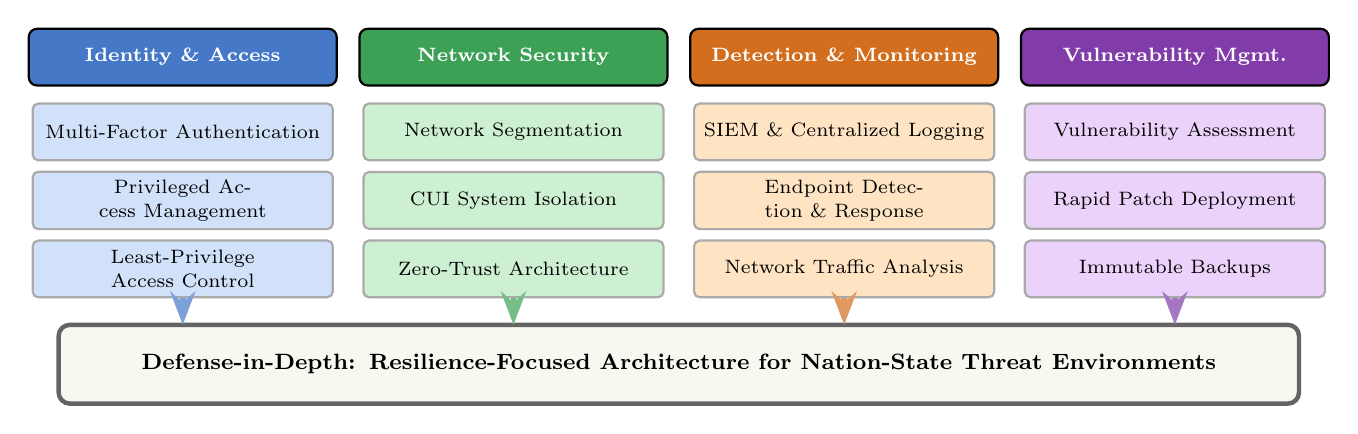
\begin{tikzpicture}[
  font=\fontsize{7pt}{9pt}\selectfont,
  >=Stealth,
  hdr/.style={
    rectangle, rounded corners=3pt,
    minimum width=3.8cm, minimum height=0.72cm,
    text centered, text width=3.7cm,
    draw, thick, text=white,
    font=\fontsize{7.5pt}{9pt}\selectfont\bfseries,
    inner sep=3pt
  },
  itm/.style={
    rectangle, rounded corners=2pt,
    minimum width=3.8cm, minimum height=0.72cm,
    text centered, text width=3.6cm,
    draw=cgray!55, thick,
    font=\fontsize{6.8pt}{8.5pt}\selectfont,
    inner sep=3pt
  },
  carr/.style={-{Stealth}, line width=2.0pt},
  ban/.style={
    rectangle, rounded corners=4pt,
    minimum width=15.6cm, minimum height=1.0cm,
    text centered, text width=15.4cm,
    draw=cgray, ultra thick, fill=clgy,
    font=\fontsize{8.5pt}{10pt}\selectfont\bfseries,
    inner sep=5pt
  }
]

%% ── Column x-centres ─────────────────────────────────────────────────────────
\def\ca{0}
\def\cb{4.2}
\def\cc{8.4}
\def\cd{12.6}

%% ── Row y-positions ──────────────────────────────────────────────────────────
\def\yh{0}      %% headers
\def\ya{-0.95}  %% item row 1
\def\yb{-1.82}  %% item row 2
\def\yc{-2.69}  %% item row 3
\def\yd{-3.90}  %% banner

%% ════ Column 1 — Identity & Access (blue) ════════════════════════════════════
\node[hdr, fill=cblue]    at (\ca,\yh)  {Identity \& Access};
\node[itm, fill=clb]      at (\ca,\ya)  {Multi-Factor Authentication};
\node[itm, fill=clb]      at (\ca,\yb)  {Privileged Access Management};
\node[itm, fill=clb] (c1) at (\ca,\yc)  {Least-Privilege Access Control};

%% ════ Column 2 — Network Security (green) ════════════════════════════════════
\node[hdr, fill=cgreen]   at (\cb,\yh)  {Network Security};
\node[itm, fill=clg]      at (\cb,\ya)  {Network Segmentation};
\node[itm, fill=clg]      at (\cb,\yb)  {CUI System Isolation};
\node[itm, fill=clg] (c2) at (\cb,\yc)  {Zero-Trust Architecture};

%% ════ Column 3 — Detection & Monitoring (orange) ════════════════════════════
\node[hdr, fill=corange]  at (\cc,\yh)  {Detection \& Monitoring};
\node[itm, fill=clo]      at (\cc,\ya)  {SIEM \& Centralized Logging};
\node[itm, fill=clo]      at (\cc,\yb)  {Endpoint Detection \& Response};
\node[itm, fill=clo] (c3) at (\cc,\yc)  {Network Traffic Analysis};

%% ════ Column 4 — Vulnerability Management (purple) ══════════════════════════
\node[hdr, fill=cpurple]  at (\cd,\yh)  {Vulnerability Mgmt.};
\node[itm, fill=clp]      at (\cd,\ya)  {Vulnerability Assessment};
\node[itm, fill=clp]      at (\cd,\yb)  {Rapid Patch Deployment};
\node[itm, fill=clp] (c4) at (\cd,\yc)  {Immutable Backups};

%% ════ Bottom banner (centred between columns 1 and 4) ════════════════════════
\node[ban] (ban) at ({(\ca+\cd)/2}, \yd)
  {Defense-in-Depth: Resilience-Focused Architecture for Nation-State Threat Environments};

%% ════ One thick column arrow each → banner ═══════════════════════════════════
\draw[carr, color=cblue!70]   (c1.south) -- (\ca,  {\yd+0.5});
\draw[carr, color=cgreen!70]  (c2.south) -- (\cb,  {\yd+0.5});
\draw[carr, color=corange!70] (c3.south) -- (\cc,  {\yd+0.5});
\draw[carr, color=cpurple!70] (c4.south) -- (\cd,  {\yd+0.5});

\end{tikzpicture}
\caption{Proposed architectural security framework for resource-constrained defense
  contractors. Four control pillars---Identity \& Access, Network Security, Detection
  \& Monitoring, and Vulnerability Management---converge into a defense-in-depth,
  resilience-focused architecture against nation-state threats.}
\label{fig:framework}
\end{figure*}

\subsection{Identity Governance and Access Management}

MFA should be required for all email, file server, VPN, and privileged account access;
hardware tokens or authenticator apps are preferred over SMS~\cite{cisa2024russia}.
Privileged Access Management (PAM) provides just-in-time privilege elevation,
session recording, automated service account password rotation, and restriction of
administrative tool access---directly increasing exploitability friction.
Access control policies should enforce role-based access to shared mailboxes, data loss
prevention (DLP) rules preventing bulk export, and least-privilege file share
permissions with regular recertification.

\subsection{Network Segmentation and Isolation}

Network zones should separate CUI systems (email, file servers) from corporate
workstations, guest/BYOD access, management infrastructure, and DMZs. Default-deny
firewall policies with inter-zone inspection and full logging contain lateral movement,
directly addressing the exploitability dimension~\cite{rockwell2024}. Micro-segmentation
further isolates email servers from file servers, restricts database access to
application servers, places backup systems on separate segments, and routes
administrative access through jump servers.

\subsection{Enhanced Visibility and Monitoring}

Log sources should include Windows Event Logs (authentication, process creation,
PowerShell), email and file server access logs, firewall and VPN logs, EDR telemetry,
and cloud service logs. Key detection use cases include: failed authentication and
impossible travel anomalies; privilege escalation attempts; unusual data access volume;
large data transfers and unusual protocol use. Behavioral analytics identifying anomalies
directly improves the discoverability dimension~\cite{guidehouse2023}.

\subsection{Vulnerability and Patch Management}

A risk-based prioritization framework: \emph{critical} (remotely exploitable on
internet-facing or CUI systems) → patch within 72 hours; \emph{high} (privilege
escalation or known active exploitation) → 7 days; \emph{medium} (CUI or
internet-facing) → 30 days; \emph{low} → 90 days. Systematic patching directly reduces
exploitability by eliminating weaknesses nation-state actors routinely exploit.

\subsection{Email and File Server Security}

Anti-phishing controls include link sandboxing, email authentication
(DMARC, SPF, DKIM), external email banners, and phishing simulation exercises with
targeted training on job offer scams (Lazarus TTP). File server controls include access auditing, CUI access alerting, and monitoring
for unusual bulk copy operations. Backup strategy requires automated daily backups to
immutable or air-gapped storage with regular restoration testing---reducing damage
potential by enabling recovery from destructive attacks, though not preventing
espionage~\cite{networkcomputing2024}.

%%──────────────────────────────────────────────────────────────────────────────
\section{Implementation Roadmap and Prioritization}
%%──────────────────────────────────────────────────────────────────────────────

\textbf{Phase 1 (Months 1--3, Foundation).} Deploy MFA for email and VPN; implement
basic anti-phishing controls; initiate vulnerability scanning; establish backup
verification; conduct phishing and job-offer-scam awareness training; patch critical
and high vulnerabilities; enable basic logging on critical systems.

\textbf{Phase 2 (Months 4--6, Enhanced Detection).} Deploy SIEM or MDR service; deploy
EDR on all servers and privileged user workstations; complete MFA across organization;
implement PAM for administrative accounts; deploy conditional access policies.

\textbf{Phase 3 (Months 7--12, Segmentation).} Design and implement network segmentation
with CUI zone isolation; deploy jump servers for administrative access; formalize patch
management with SLAs; conduct incident response tabletop exercises.

\textbf{Phase 4 (Months 13--24, Maturity).} Implement threat hunting; deploy DLP across
email, endpoints, and file servers; integrate industry threat intelligence sharing;
conduct regular penetration testing and threat model reassessment.

\begin{table}[h]
\caption{Estimated Investment Ranges for Small Defense Contractors (50--200 employees).}
\label{tab:costs}
\small
\begin{tabularx}{\columnwidth}{@{}Xl@{}}
\toprule
\textbf{Capability} & \textbf{Annual Cost} \\
\midrule
MFA (cloud-based)           & \$5K -- \$15K    \\
EDR Platform                & \$20K -- \$50K   \\
SIEM / MDR Service          & \$50K -- \$150K  \\
PAM Solution                & \$15K -- \$40K   \\
Vulnerability Management    & \$10K -- \$30K   \\
Security Awareness Training & \$5K -- \$15K    \\
Incident Response Retainer  & \$20K -- \$50K   \\
Network Segmentation (one-time) & \$30K -- \$100K \\
Consulting Support          & \$50K -- \$150K  \\
\midrule
\textbf{Total Year 1}  & \textbf{\$205K -- \$600K} \\
\textbf{Ongoing Year 2+} & \textbf{\$175K -- \$450K} \\
\bottomrule
\end{tabularx}
\end{table}

These estimates reflect that meaningful nation-state defense requires investment of
2--5\% of revenue for typical small defense contractors, directly supporting CMMC
contract eligibility and reducing catastrophic breach risk.

%%──────────────────────────────────────────────────────────────────────────────
\section{Discussion}
%%──────────────────────────────────────────────────────────────────────────────

\subsection{DREAD Methodology Limitations}

DREAD has inherent limitations: scoring involves judgment and different assessors may
assign different scores; arithmetic averaging can mask extremes (catastrophic-damage,
low-probability threats may merit special treatment); the dynamic threat landscape
requires periodic reassessment; and DREAD captures individual threats rather than
cumulative risk from multiple vectors. Despite these limitations, DREAD's structured
quantitative approach enables consistent, communicable risk assessment---particularly
valuable for resource-constrained organizations requiring clear prioritization.

\subsection{Threat Modeling as Strategic Tool}

DREAD scores translate technical threats into metrics non-technical leadership can engage
with: an ``8.0/10 high-risk score'' is more actionable than ``nation-states are a
concern.'' Quantification supports cost-benefit analysis, links specific investments to
risk reduction, demonstrates due diligence for CMMC compliance, and provides an audit
trail of risk-informed decision making. For organizations with limited budgets, threat
modeling ensures highest-scoring threats receive priority attention and controls
addressing multiple high-scoring dimensions provide best return.

\subsection{Future Threat Considerations}

AI-generated phishing content is more convincing and scalable, automated vulnerability
discovery accelerates exploit development, and deepfake technology enables sophisticated
impersonation---each likely increasing exploitability and reproducibility scores in
future assessments. Supply chain attack evolution following SolarWinds suggests increased
focus on managed service providers and cloud service dependencies. For data with
long-term sensitivity (decades-long defense programs), ``harvest now, decrypt later''
strategies targeting encrypted data today for future quantum decryption represent an
emerging structural risk requiring migration to quantum-resistant
cryptography~\cite{nist2024sp800171}.

%%──────────────────────────────────────────────────────────────────────────────
\section{Conclusion}
\sloppy
%%──────────────────────────────────────────────────────────────────────────────

This research demonstrates how small defense contractors can apply structured threat
modeling to assess and respond to nation-state cyber threats despite significant resource
constraints. Through DREAD analysis of GRU and Lazarus Group threats to email and file
server infrastructure, we quantified a high-risk scenario (8.0/10) driven by
catastrophic damage potential, organization-wide impact, and moderate-high exploitability.

Six critical findings emerge. Nation-state threats to small defense contractors are
severe and realistic---both GRU and Lazarus have demonstrated willingness and capability
to target organizations matching this profile. Email and file server compromise provides
catastrophic adversary advantage, with damage and affected-users scores of 9/10
confirming their status as crown jewel targets. Common security weaknesses dramatically
increase exploitability---much adversary success derives from predictable gaps in patch
management, authentication, and monitoring. Detection is challenging but achievable
through behavioral analytics and threat intelligence integration. Resource-constrained
organizations can meaningfully improve security through the phased roadmap, committing
2--5\% of revenue. Threat modeling provides strategic value beyond technical
assessment, enabling risk communication, investment justification, and prioritization.

The proposed architectural framework emphasizes resilience over prevention: assuming
compromise will occur and designing systems to limit damage, detect intrusions, and
recover operations. This shift---from ``keeping adversaries out'' to ``limiting
adversary advantage when they get in''---aligns with modern zero-trust principles and
acknowledges the sophistication of nation-state adversaries. Through systematic threat modeling,
strategic investments in highest-priority controls, and continuous improvement,
resource-constrained defense contractors can navigate the threat landscape while
supporting national security objectives.

%%──────────────────────────────────────────────────────────────────────────────
\sloppy
\bibliographystyle{ACM-Reference-Format}
\begin{thebibliography}{99}

\bibitem{case2021ukraine}
D.~U.~Case, ``Analysis of the cyber attack on the Ukrainian power grid,''
\textit{E-ISAC}, 2021.

\bibitem{chang2025mind}
V.~Chang et al., ``Mind the gap: Balancing organizational resources to combat
cybersecurity challenges,'' \textit{IEEE Trans.\ Eng.\ Mgmt.}, vol.~72, no.~1,
pp.~234--249, 2025.

\bibitem{cisa2024nationstate}
CISA, ``Nation-state cyber actors,'' 2024.
\url{https://www.cisa.gov/topics/cyber-threats-and-advisories/nation-state-cyber-actors}

\bibitem{cisa2024russia}
CISA, ``Russian state-sponsored cyber actors gain network access,'' Alert AA22-074A, 2024.

\bibitem{cisa2024volt}
CISA, ``PRC state-sponsored actors compromise and maintain persistent access to U.S.
critical infrastructure,'' Advisory AA24-038A, 2024.

\bibitem{crowdstrike2024global}
CrowdStrike, ``2024 Global Threat Report,'' Feb.~2024.
\url{https://www.crowdstrike.com/wp-content/uploads/2024/02/crowdstrike-2024-global-threat-report-executive-summary.pdf}

\bibitem{dod2024cmmc}
U.S.\ DoD, ``Cybersecurity Maturity Model Certification (CMMC) Program,'' 2024.

\bibitem{gao2021defense}
U.S.\ GAO, ``Weapon Systems Cybersecurity: DOD Just Beginning to Grapple with Scale of
Vulnerabilities,'' GAO-21-288, 2021.

\bibitem{greenberg2019notpetya}
A.~Greenberg, ``The untold story of NotPetya,'' \textit{Wired}, Aug.~2019.

\bibitem{greenberg2021sandworm}
A.~Greenberg, \textit{Sandworm}. Anchor Books, 2021.

\bibitem{guidehouse2023}
Guidehouse, ``Building Resilience in Security Architecture,'' Dec.~2023.
\url{https://guidehouse.com/insights/advanced-solutions/2023/building-resilience-in-security-architecture}

\bibitem{kelly2023practical}
D.~Kelley and E.~Moyle, \textit{Practical Cybersecurity Architecture}. Packt, 2023.

\bibitem{mandiant2023china}
Mandiant, ``China Nexus Cyber Espionage: Threat Overview,'' 2023.

\bibitem{mandiant2023iran}
Mandiant, ``Iranian Cyber Threat Overview,'' 2023.

\bibitem{mascellino2025dreamjob}
A.~Mascellino, ``Lazarus Group's Operation Dream Job targets European defense firms,''
\textit{Infosecurity Magazine}, Oct.~2025.
\url{https://www.infosecurity-magazine.com/news/lazarus-groups-operation-dreamjob/}

\bibitem{meier2003dread}
J.~D.~Meier et al., ``Improving Web Application Security: Threats and Countermeasures,''
Microsoft Corporation, 2003.

\bibitem{mitre2022supply}
MITRE, ``Deliver Uncompromised: A Strategy for Supply Chain Security,'' 2022.

\bibitem{nara2024cui}
NARA, ``Controlled Unclassified Information (CUI) Registry,'' 2024.
\url{https://www.archives.gov/cui}

\bibitem{networkcomputing2024}
Network Computing, ``Structured for Success: 4 Architectural Pillars of Cyber
Resilience,'' Nov.~2024.

\bibitem{nist2023smallbiz}
NIST, ``Small Business Cybersecurity Corner,'' 2023.
\url{https://www.nist.gov/itl/smallbusinesscyber}

\bibitem{nist2024sp800171}
NIST, ``Protecting CUI in Nonfederal Systems,'' SP~800-171 Rev.~3, 2024.

\bibitem{rockwell2024}
Rockwell Automation, ``Compensating Controls in OT Security,'' Mar.~2024.

\bibitem{shostack2014threat}
A.~Shostack, \textit{Threat Modeling: Designing for Security}. Wiley, 2014.

\bibitem{smith2021solarwinds}
B.~Smith, ``A Moment of Reckoning: The Need for a Strong and Global Cybersecurity
Response,'' \textit{Microsoft On the Issues}, Dec.~2021.

\bibitem{ucedavelez2015risk}
T.~UcedaVelez and M.~M.~Morana, \textit{Risk Centric Threat Modeling}. Wiley, 2015.

\end{thebibliography}

\end{document}
